\documentclass[preprint,11pt,3p]{article}

\usepackage{tocloft}
\usepackage{color}
\usepackage{hyperref}
\usepackage{graphicx}

\renewcommand{\cftsecleader}{\cftdotfill{\cftdotsep}}
\renewcommand{\abstractname}{Executive Summary}

\hypersetup{
	colorlinks = true,
	citecolor = black,
	filecolor = black,
	linkcolor = black,
	urlcolor = black,
}

\title{Cruise Control Software Development Version 0.03}

\author{
Eric Altenburg, Michael McCreesh, Hamzah Nizami, Constance Xu}
	
\date{
	Stevens Institute of Technology\endgraf\bigskip
	CS 347 — Software Development Process\endgraf\bigskip
	\textit{We pledge our honor that we have abided by the Stevens Honor System.}}

\begin{document}

\maketitle
\newpage

\tableofcontents
\newpage

\begin{abstract}
	Team Mike is a startup initiative aimed at solving problems that come to light as
society begins to adopt new technologies. One of which pertains to autonomous
driving and “smart cars” as they are beginning to break into the automobile
market more and more every year with examples such as Tesla and Ford. In a
perfect world, if every driving car were to be a smart car with “autopilot,” then
it would make sense for each of them to communicate cruise control data with
each other to reduce traffic build-up and make traveling more efficient. Through
rotational leadership on a monthly basis, each team member possesses a set of
distinct skills that can translate to highly efficient work sessions. Aside from
developing a traditional cruise control, it can sense other cars’ locations and
communicate information, which will allow autonomous cars to fully achieve
their potential within a growing technologically advanced society.
\end{abstract}

\section {Introduction}
The past century has seen an explosion of innovation on a scale never before seen
in human history. The rapid development and refinement of a myriad of motor
technologies catalyzed the innovation process by allowing ideas to transfer at
rates never before seen. With the constraint of distance loosening thanks to
every iteration of the automobile, people have been granted more freedom to
do what they please. While the automobile has enhanced society in several
ways, there are some glaring problems that need to be addressed to continue
the current rate of human progress and innovation. One of the biggest problems
is driver fatigue, which is responsible for approximately 72,000 crashes annually.
Programming the automobile to be reliably autonomous to a degree is one way
to circumvent the issue of driver fatigue and making roads safer. That’s exactly
what cruise control aims to do. By moderating the speed of the vehicle by itself,
cruise controls aim to lessen the effects of driver fatigue on the road. However,
the technology is not perfect, and Team Mike aims to resolve that by creating
the perfect cruise control system. \par
When it was implemented in 1958, cruise control was suitable for that era,
however, as technology continually improves, the embedded software must as
well. With more advanced sensors, it is now possible to be able to sense where
surrounding vehicles are at all times, and with this, the overall safety of the
passenger can be increased while allowing them to have a more enjoyable ride.
For longer car trips, it does not make sense for users to constantly accelerate
and decelerate for several miles; this is where cruise control comes in. By being
able to set the speed, the user is now able to accurately set and maintain the
speed they wish to without having to constantly intervene which, over time,
would cause less harm to the vehicle as variable speed and RPMs are not as
desirable as that of near-constant. \par
Our group intends to use an Agile method to implement our version of cruise
control. This would encourage code sprints in two-week lengths where work
will be divided into smaller sections and distributed based on each members’
strengths. The Agile method may vary as to which one we specifically choose
but regardless, this project will not come to fruition using Waterfall or other
methods. The way that we are going to organize our group is through weekly
meetings and ensuring that everyone knows their tasks for the week. These
weekly meetings can also serve as a place where team members mention any
obstacles that have come in their way when trying to resolve a problem, and
also serve as a time where the team as a collective can try to think of solutions
around those obstacles. We also plan on giving real-time updates about any
progress made through Slack in order to ensure all members of the team are
equipped with the most recent developments of the project. We also intend on
using Java or C++ to implement our cruise control system. We believe that the
high-performance Java provides and the fact that its part of the Object-Oriented
Programming (OOP) paradigm makes it perfect for embedded systems. \par
There are a plethora of features that make up cruise control. As most cruise
controls are seen on vehicles, there are generally a few buttons: increase speed
(and sometimes decrease speed) and the button that starts cruise control. Once
cruise control is set, the user then has the ability to increase, decrease, or
maintain the speed of a vehicle. Furthermore, if the user presses on the brake,
then cruise control is automatically deactivated. The system also allows for the
operator of a vehicle to manually deactivate it. A useful feature that we intend
on implementing is maintaining a safe distance away from the car in front of
the vehicle, hence creating more of an autopilot mode as opposed to a cruise
control scenario. \par
To successfully implement the features of maintaining a steady speed and a
safe distance away from other cars, there are certain requirements to fulfill. At a
high level, proper hardware with fast, reliable sensors is critical for this project.
Furthermore, lives are fundamentally dependent on this product and therefore
it requires software that is error-resistant and thus a strong development and
QA (quality assurance) team. In addition, the software must also perform it’s
expected tasks of moderating speed, maintaining a safe distance and switching
back control to the driver when prompted to quickly. Having a cruise control
software that is slow would be ineffective, so speed and accuracy are critical
requirements for the software as well as the hardware. This is a mission-critical
system because if it were to fail, it would put the lives of people in danger.

\newpage
\section{Requirements}

\subsection{Input}
\begin{enumerate}
	\item The power button that allows for the state of the system to change
		\begin{enumerate}
			\item From on to off or vice versa
		\end{enumerate}
	\item Button to set speed %Are these the same thing
	\item A button to select either accelerate or decelerate
	\item Have the brake to be an alternate method of turning off the system
	\item If the entire car turns off, then a signal will be sent to turn off the system that is separate from the car shutdown
	\item RPM (Rotations Per Minute) sensor should be connected to the front axle and able to take readings for accurate speed calculations. 
	\item RADAR sensor must be able to detect nearby vehicles/obstacles to avoid collision. %Do we really wanna do this
	\item Engine sensor must be able to take input from the engine to tell the cruise control system to turn on or off.
	\item Brake pedal sensor must be able to take input from user to stop when pressed and keep going when released.
\end{enumerate}

\subsection{Output}
\begin{enumerate}
	\item Keep a log of activity to help debug in the event of a malfunction
	\item For every speed increase made by the user in cruise control, a small haptic feedback accompanied by a visual indication by the software is necessary. This is so that the user minimizes their own human error. So, every time you increase the speed, you can see the cruise control speed on the car menu increasing by however much the user wants it to.
	\item The system displays successful activation or deactivation within a fast time frame, less than ten milliseconds. *Numbers are subject to change depending on how inputs are received from surrounding system, but are expected to be in around that same ballpark.*
	\item Keep a log of every time cruise control is used and at what speed
	\item This module must be able to do what the user wants within a fast time frame, less than ten milliseconds. *Numbers are subject to change depending on how inputs are received from surrounding system, but are expected to be in around that same ballpark.*
	\item Once the entire system is turned on, cruise control must be readily available. The engine sensor must be able to understand that the engine is on and tell the cruise control system that, if the user so wishes, it must activate. 
	\item With all the inputs it is taking from all the sensors, the software must be able to deliver the desired output for each function in a less than 15 milliseconds. So, the RADAR sensor must be able to tell the software that a car is nearby, and the car must do the appropriate action. The brake pedal sensor must be able to tell the software that the user has stopped, and stop the cruise control. *Numbers are subject to change depending on how inputs are received from surrounding system, but are expected to be in around that same ballpark.*
\end{enumerate}

\subsection{Functional}
\begin{enumerate}
	\item Able to increase and decrease the speed by 1 mph
	\item Able to switch cruise control on or off provided the engine is on
	\item Able to read sensor data and act accordingly %and do what
	\item Only allow the cruise control to be activated when at a minimum speed of 25 mph %What if we set speed and and set speed below this
	\item Maximum speed that cruise control can be activated is around 125 mph. 
	\item Given a speed by the user, the cruise control software maintains the speed provided
\end{enumerate}

\subsection{Security}
\begin{enumerate}
	\item No external interface to reduce potential tampering. This applies to both the hardware such as sensors and the general cruise control software. There would be no easy access to the cruise control hardware or software so that the likelihood of someone being able to create issues is reduced substantially. 
	\item No Internet or Bluetooth connection. This is so that no bad actors can meddle with the car's system and hence, keeps the drivers safer as cyber security becomes more of an issue.
	\item An administrator will need hardware to make changes to the mechanisms. The administrator must be authorized to make these changes and they must be a trusted third party or those who created the cruise control themselves. 
\end{enumerate}

\subsection{UML Diagram}
\begin{enumerate}
	\item An example can be seen in Figure ~\ref{fig:ccUML1}: The user has requested for the cruise control to power on, in doing so, the system provides feedback through activation of say a light on the dashboard. Then the user can set the velocity where the system will then send a request to the throttle waiting for feedback, once received, it will then request an update from the sensors for the speedometer. The same concept is used when the user would like to increase or decrease the velocity; send a request to the throttle and upon feedback, request information from the sensors for up-to-date information. For powering off, once the user either presses the brake or off button, then it will remove the set throttle request made earlier from a velocity set and then give the user feedback upon successful throttle set removal. %Replace with: General I/O for the cruise control system
		\begin{figure}[h]
			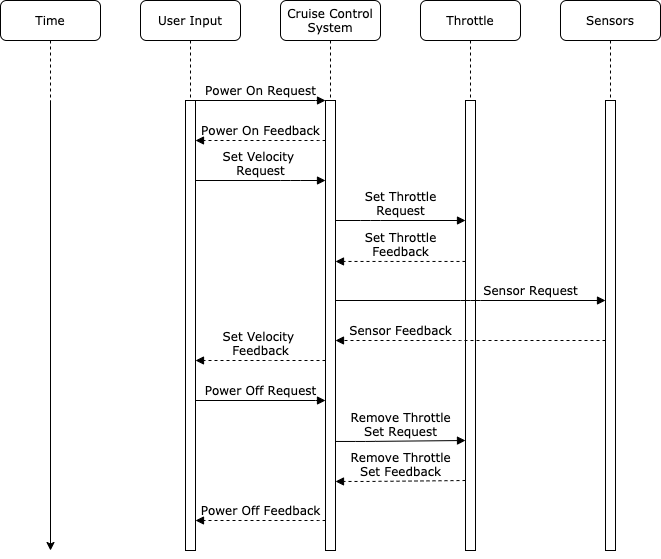
\includegraphics[width=0.9\textwidth]{images/ccUML.png}
			\caption{Sample UML diagram for cruise control activation, velocity set, and deactivation.}
			\label{fig:ccUML1}
		\end{figure}
\end{enumerate}


	


\end{document}

